\chapter{\IfLanguageName{dutch}{Stand van zaken}{State of the art}}
\label{ch:stand-van-zaken}

% Tip: Begin elk hoofdstuk met een paragraaf inleiding die beschrijft hoe
% dit hoofdstuk past binnen het geheel van de bachelorproef. Geef in het
% bijzonder aan wat de link is met het vorige en volgende hoofdstuk.

% Pas na deze inleidende paragraaf komt de eerste sectiehoofding.

% Dit hoofdstuk bevat je literatuurstudie. De inhoud gaat verder op de inleiding, maar zal het onderwerp van de bachelorproef *diepgaand* uitspitten. De bedoeling is dat de lezer na lezing van dit hoofdstuk helemaal op de hoogte is van de huidige stand van zaken (state-of-the-art) in het onderzoeksdomein. Iemand die niet vertrouwd is met het onderwerp, weet nu voldoende om de rest van het verhaal te kunnen volgen, zonder dat die er nog andere informatie moet over opzoeken \autocite{Pollefliet2011}.

% Je verwijst bij elke bewering die je doet, vakterm die je introduceert, enz. naar je bronnen. In \LaTeX{} kan dat met het commando \texttt{$\backslash${textcite\{\}}} of \texttt{$\backslash${autocite\{\}}}. Als argument van het commando geef je de ``sleutel'' van een ``record'' in een bibliografische databank in het Bib\LaTeX{}-formaat (een tekstbestand). Als je expliciet naar de auteur verwijst in de zin, gebruik je \texttt{$\backslash${}textcite\{\}}.
% Soms wil je de auteur niet expliciet vernoemen, dan gebruik je \texttt{$\backslash${}autocite\{\}}. In de volgende paragraaf een voorbeeld van elk.

% \textcite{Knuth1998} schreef een van de standaardwerken over sorteer- en zoekalgoritmen. Experten zijn het erover eens dat cloud computing een interessante opportuniteit vormen, zowel voor gebruikers als voor dienstverleners op vlak van informatietechnologie~\autocite{Creeger2009}.

To get a grasp on how quantum computers work, a base knowledge of quantum physics is needed.
The basis of the operation of quantum computers mainly lies in two quantum mechanical phenomena: superposition and entanglement.
These two phenomena combined with the limit that all operations used in the computing makes a quantum computer work like it works.
Yen the computer can't do things on it's own, it has the need of an algorithm that tells it what to do and when to do it.
In this case a classic algorithm just won't do the trick, since they don't manipulate qubits. A higher 'level' of algorithm is needed: a quantum algorithm.

\section{Quantum mechanics} \label{quantum mechanics}
\epigraph{If you are not completely confused by quantum mechanics, you do not understand it.}{\textit{Niels Bohr}}

In this section, the fundamentals of quantum physics used in a quantum computer will be laid out.
This will only focus on the core items and won't be as in depth. If there is a need in a deeper understanding, don't hesitate to read the papers and articles used in this section.
To understand the basics of quantum computing, the next mathematical things should be familiar:

\begin{itemize}
    \item linear algebra
    \item complex numbers
    \item matrices
\end{itemize}

For more information on the mathematical side of this study, look into the book of \textcite{bernhardt_2019}.

\subsection{Dirac Notation} \label{Dirac}
Also known as the bra-ketnotation, is a commonly used notation in quantum mechanics is the Dirac notation to denote vectors \autocite{Dirac_Notation2020}.
As can be read in the Microsoft\textregistered documentations on quantum computing, the notation of vectors can be real cumbersome \autocite{Microsoft_Dirac}. To make these notations easier to read and just keep them simple, the Dirac notation is used.

Take a vector $\vec{x}$ equal to $\begin{bmatrix}
    1 & 0 
\end{bmatrix}$.
Since this is a row matrix it can be easily written in the Dirac notation as a bra: $\bra{x}$. The same can be done for column matrices, these would become kets. As an example:
vector $\vec{y}$ = $\begin{bmatrix}
    1 \\
    0
\end{bmatrix}$ can be written as the following ket $\ket{y}$.
The Dirac notation can also be used for the inner product of vectors: the product of $\vec{x}$ and $\vec{y}$ becomes the braket $\Braket{x|y}$ as can be seen on \textcite{Dirac_Notation2020} as well on \textcite{Microsoft_Dirac}.

\subsection{Superposition} \label{superposition}
Superposition is know by most people through an experiment done by a famous Austrian scientist: Erwin Schrödinger.
The experiment itself was not really executed, but was a thought-experiment. In the experiment one would take a cat and place it in a box or bunker. 
In it there is a barrel with gunpowder or poison gas which would kill the cat 50 precent of the times. So, if the experiment was done a thousand times in 500 cases the cat would have died.
Quantum physics state that as long as the box or the bunker isn't opened the cat is in a superposition: it is death as well it is alive.
When the box or bunker is opened, the state of the cat is known \autocite{Villars_1986}.
Superposition is a state where an object has the possibility of being in either one of the base states. Only by taking a measurement on the object, it's state is defined.
To get a more mathematical view on superposition, the following principle is stated in the book by \textcite{Hidary_2019}:
"The linear combination of two or more state vectors is another state vector in the same Hilbert space \footnote{A hilbert space is a complex vector space with an inner product. \autocite{Griffiths2014}} and describes another state of the system."
Another commonly used example of superposition is the polarization of light. The light we see, coming from the sun or lamps, has no particular direction of polarization.
Light is in a superposition: there is a mix of vertically and horizontally polarized light. But, if needed, one particular polarization can be filtered.
By letting the light passing through a polarization film, this filters the light with a polarization in one particular axis parallel of that of the film, can one particular direction be seen.
A commonly know polarization filter is a pair sunglasses.

\begin{figure} [h]
    \centering
    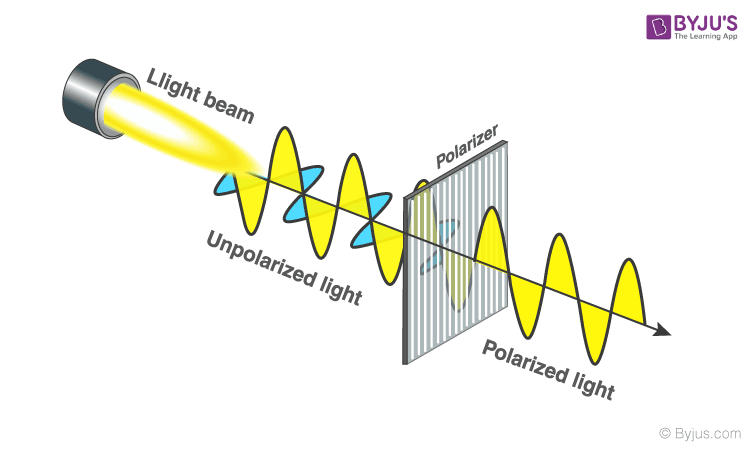
\includegraphics[width=\textwidth]{img/Polarization-of-Light-2.png}
        \caption{Polarization of light}
        \label{fig:polarization}
    \href{https://byjus.com/physics/polarization-of-light/}{Source: Byju's}

\end{figure}


\subsection{Quantum entanglement} \label{quantum entanglement}
What \textcite{Einstein} once described in a letter to Daniel M. Lipkin as "a little system of delusion of an exceedingly intelligent paranoiac concocted of incoherent elements of thought", is now a well-know fact in the quantum mechanical world.
Quantum entanglement is the phenomenon where two or more quantum objects are coupled together, they are in a state where they live together.
Or as described in in the book by \textcite{Hidary_2019}: "Two systems are in a special case of a quantum mechanical superposition called entanglement if the measurement of the one system is correlated with the state of the other system in a way that is stronger than the correlations in the classical world.".
Even though the objects are entangled, they are not physically bound to eachother. So one object could be on the north pole and the other one on the south pole.
In the paper written by Einstein, Podolsky and Rosen they describe that if one of 2 entangled particles is measured, it triggers a correlated state of the second particle \autocite{EPR}.


\section{Computing} \label{computing}
There are a lot of different types of computers: desktops, laptops, quanta and even servers are in fact just computers that are specialised in doing something specific.
To understand how a quantum computer works, one should start at the base of that: the classical computer. Even though almost everyone uses a computer on a daily basis, not many people know how it works.


\subsection{Classical computer} \label{classical computer}
A computer consists two main parts: software and hardware. The hardware are the physical parts that make the computer: like a central processing unit (or CPU in short), Random Access Memory (RAM) and many other parts.
Software on the other hand are the programs that run on the pc. Think of the Operating System (OS) and programs like Word, PowerPoint and may others.


\subsubsection{Hardware} \label{hardware}
A motherbord, CPU, RAM, hard drive and a power supply are the basics every pc should have in order to work.
Add-ons like a Graphical processing unit (GPU or grapic card), a nice case to put everything in, a network card and cooling are nice to have and can help make the pc run better or faster.
The central processing unit is the brain of the computer. It makes all the calculations that should be done.
Then there is the motherboard. This could be seen like the nervous system of the pc: everything is connected to it and it lets every part speak with eachother.
Whilst the CPU is calculating things, some of the calculations should be stored for a while and this is put in the RAM. Random access memory is volatile which means that when the pc is shut down everything stored on it is lost.
That's why there is a hard disk. The hard drive stores all the items that should be stored for a longer time. So when a word document is being written it starts in the RAM, but the second the file is saved it is transferred to the hard disk.
Since every component of a computer works on chips that are based on voltages, there is a need for electricity. This is where the power supply (sometimes shortened as PSU) comes in handy. This takes in the power from an outlet and converts it to the right amounts so the components won't get fried.
There is also hardware that is connected to the computer. This lets somebody work with it. Examples of external hardware are a monitor, keyboard and mouse, a printer, etc.
These were the basics explained so that the pc can run, but there are many other part where the info from can be found on \cite[https://edu.Fcfglobal.org/en/computerbasics/]{ComputerBasics}.

\begin{figure} [h]
    \centering
    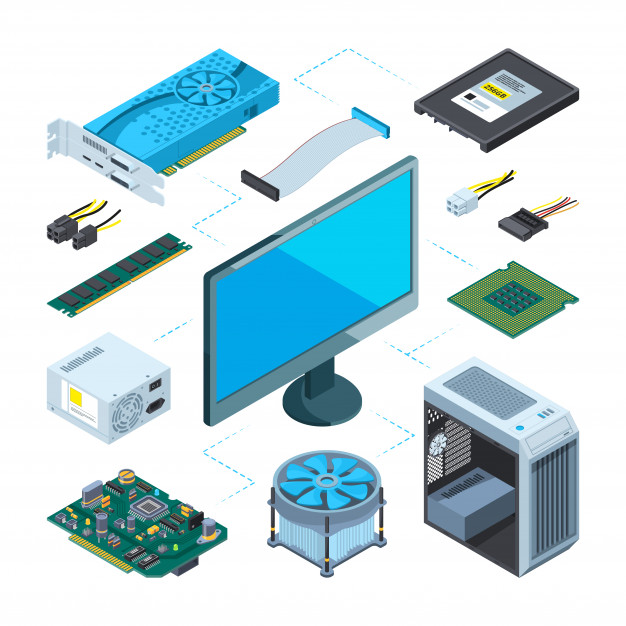
\includegraphics[width=\textwidth]{img/hardware.jpg}
        \caption{Hardware components}
        \label{fig:hardware}
        \href{https://nl.freepik.com/premium-vector/computer-hardware_4618150.htm}{Source: Freepik}
\end{figure}

The components from top to bottom and left to right: GPU, power cable, RAM, PSU, motherboard, internal cable, monitor, a fan, hard drive, data cable, CPU and the case.


\subsubsection{Software} \label{software}
Software is everything that runs on the hardware that is just described. It is an instructionlist: it tells the hardware what to do, how to do it and even when to do it \autocite{software}.
The most underlying software program is the operation system. This tells the hardware how the computer works. On top of the OS additional programs can be installed to do a variety of tasks: a text processor like word, a browser to access the internet like google chrome and many more.


\subsubsection{Operation} \label{working}
A calculation in the CPU has 3 stages: fetch, decode, execute \autocite{CPU}.
In the fetch-stage the CPU grabs an instruction from the RAM. It then decodes this instruction in de decode-stage and finally when it exacly knows what the instruction means, it executes this in the execute-stage.
The CPU is made up of several billions of transistors. A tranistor is an on-off switch that, when in the on state, lets current pass through or it stops it from flowing.
To represent data bits are used. This has two values: one or zero\autocite{bit}. In the case of computers this would translate to: there is a voltage detected in the transistor or there is not.
When there are two bits the calculations can start. Calculation is nothing more than taking two bits, insert those in a logical gate and the answers is spat out.
There are six logic gates: AND, OR, EXOR, NAND, NOR and EXNOR \autocite{gates}. Then there's also the inverter or the NOT-gate and a buffer, but the buffer won't be explained here.

\begin{figure} [h]
    \centering
    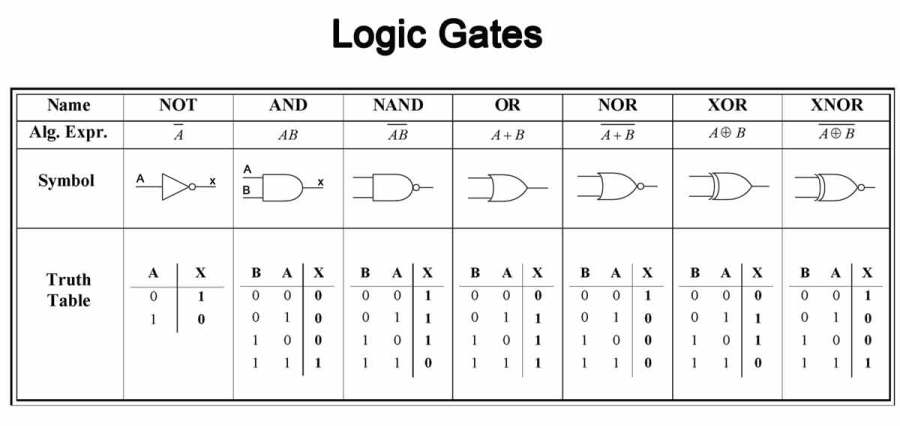
\includegraphics[width=\textwidth]{img/gates.jpg}
        \caption{Logic gates}
        \label{fig:logicGates}
        \href{https://frankcomputerscience.wordpress.com/chapter-3/}{Source: Frank Computer Science}
\end{figure}

This all means that to make faster pc's, the CPU's have to be faster. And this can only be done by placing more transistors on the CPU, because more transistors equals more calcuations.
At this moment, the amount of transistors that can be put on a chip is still rising. This is defined by \textcite{Moore1965}'s law: it started out with every year the amount doubles. But since they are getting closer to the physical bounds, this changed to every two years.


\subsection{Quantum computer} \label{quantum computer}
The big difference between the classical computer and a quantum computer is the unit of a calculation: quantum computers don't use bits but use qubits.
It is the qubit that allows to do faster calcuations because of it's quantum mechanical nature.


\subsubsection{The qubit} \label{qubit}
A qubit is the analogue of the classical bit. It too has 2 states: $\ket{0}$ and $\ket{1}$, but it can be in a linear combination of those 2 base states called the superposition \autocite{thequbit}.
\begin{equation}
    \ket{\phi} = \alpha * \ket{0} + \beta * \ket{1}
\end{equation}
This is the representation of a superposition, where $\alpha$ and $\beta$ are probability amplitudes(complex numbers) used to calculate the probability density.


The state of a qubit can also be represented visually by using the bloch sphere. The bloch sphere represents the pure states \footnote{A pure state of a system is a state that cannot be represented by a mixture of other states as can be seen in the proof of that theorem in \textcite{Ballentine2014}} of a 2-level quantum system on the surface of the sphere, and represents mixed states in it's interiour.
There are six commonly know base states on the bloch sphere:

\begin{itemize}
    \item On the Z-basis
        \begin{itemize}
            \item $\ket{0}$
            \item $\ket{1}$
        \end{itemize}
    \item On the X-basis
        \begin{itemize}
            \item $\ket{+} = \frac{\ket{0} + \ket{1}}{\sqrt{2}}$
            \item $\ket{-} = \frac{\ket{0} - \ket{1}}{\sqrt{2}}$
        \end{itemize}
    \item On the Y-basis
        \begin{itemize}
            \item $\ket{R} = \frac{\ket{0} + i \ket{1}}{\sqrt{2}}$
            \item $\ket{L} = \frac{\ket{0} - i \ket{1}}{\sqrt{2}}$
        \end{itemize}
\end{itemize}

Qubits can be physically implemented by many things: the polarization of photons, spin states of an atom or electron, etc \autocite{thequbit}.
As an example, let's make a qubit from the spin of an electron. It is know that the spin-state(up or down) can be changed by subjecting the electron in a magnetic field.
\textcite{Stern} found the atomic spin in their experiment in 1922. In the experiment they shot a beam of silveratoms through a magnetic field in a vacuum and 'catch' the atoms on a plate. After the experimented they looked at this plated and saw that instead of the atoms being distributed evenly on the plate, there were two big bundles.
One bundle was a bit higher than the center and one a bit lower. Knowing that a magnetic field has an influence on atoms, can be used as an advantage. To keep things short as seen in the Zeeman effect: applying an external magnetic fields ensures that the spinstate that the atom is in, is in a higher energy level(an exited state) than the other spinstate \autocite{Zeeman}.
And because atoms want to be in the lowest possible energystate(the groundstate), the atom will change its spin. 

\begin{figure} [h]
    \centering
    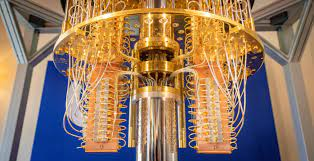
\includegraphics[width=\textwidth]{img/qcomputer.jpg}
        \caption{The cooling system of a quantum computer}
        \label{fig:Quantum computer cooling}
        \href{https://www.cnet.com/news/quantum-computing-research-helps-ibm-win-top-spot-in-patent-race/}{Source: CNET}
\end{figure}

\subsubsection{The hardware}
Since generating a qubit is very difficult work and the slightest change may give errors in calculations, there is a big need to control the outside noice.
The article by \textcite{Cooling} states that to ensure to minimize the chamce of qubits flipping between quantum states, the computer has to be cooled so that the energy level inside it is at it's lowest possible point.
Since a qubit heats up when it's used in calculations \autocite{Cooling}, the cooling must be very good. This is why they cool the qubit to temperatures around the absolute zero: zero degrees Kelvin (0°K or -273,15°C).
This cooling system is what makes the quantum computer so big, most of the photo's are in fact just the refrigerators. This is the quantum part of the quantum computer. Nut quantum computers don't work like a conventional computer, it can't connect to the internet on it's own, it can't store a lot of data on drives, etc.
To achieve this there is a need of a classical part: a classical computer that is connect to the quantum computer so that interaction with it can be achieved. This part is used to build the applications for the quantum computer \autocite{qhardware}.

The processor itself is the central part that's seen in figure \ref*{fig:Quantum computer cooling}, all the other yellow parts can be seen is the cooling system.
A quantum computer consists of 4 hardware layers: quantum data plane, control and measurement plane, control processor plane and host processor \autocite{qhardware}.

\begin{enumerate}
    \item The quantum data plane

        \quad The quantum data plane is the core of the entire computer. In this 'plane' the qubits are found.

         
    \item The control and measurement plane

        \quad The control and measurement plane is the plane where all the operations on the qubits happen. It takes the signals of the control processor plane and converts them so the operations can be executed.
        Next to converting signals to execute operations, the control and measurement plane is also in chargo of converting the signals from the measurements to binary data so that the data can be processed. As can be read in the findings on section 5.1.2 in \textcite{qhardware},
        this plane holds back the speed of the computer: the speed can not be faster than the speed to create a control signal.

    \item The control processor plane

        \quad In the control processor plane, the controlling of all the operations take place. It determines the sequence of operations on the qubits, but it doesn't execute them. It's input is the code of a program and outputs the right instructions to the control and measurement plane.

    \item The host processor

        \quad This is a classical computer that manages the 'normal' side of the operations. Here the applications are build to run on the control processor. Other functions of the host are providing storage to the quantum computing and sometimes networking.

\end{enumerate}